%-------------------------------------------------------
% SLEPc Users Manual
%-------------------------------------------------------
\chapter{\label{cap:svd}SVD: Singular Value Decomposition}
%-------------------------------------------------------

\noindent The Singular Value Decomposition (\ident{SVD}) solver object can be used for computing a partial SVD of a rectangular matrix. It provides uniform and efficient access to several specific SVD solvers included in \slepc, and also gives the possibility to compute the decomposition via the eigensolvers provided in the \ident{EPS} package.

In many aspects, the user interface of \ident{SVD} resembles that of \ident{EPS}. For this reason, this chapter and chapter \ref{cap:eps} have a very similar structure.
	
\section{\label{sec:svd}The Singular Value Decomposition}

In this section, some basic concepts about the singular value decomposition are presented. The objective is to set up the notation and also to justify some of the solution approaches, particularly those based on the \ident{EPS} object. As in the case of eigensolvers, some of the implemented methods are described in detail in the \slepc \hyperlink{str}{technical reports}.

For background material about the SVD, see for instance \citep[ch.~6]{Bai:2000:TSA}. Many other books such as \citep{Bjorck:1996:NML} or \citep{Hansen:1998:RDI} present the SVD from the perspective of its application to the solution of least squares problems and other related linear algebra problems.

The singular value decomposition (SVD) of an $m\times n$ matrix $A$ can be written as
\begin{equation}
\label{eq:svd}
A=U\Sigma V^*,
\end{equation}
where $U=[u_1,\ldots,u_m]$ is an $m\times m$ unitary matrix ($U^*U=I$), $V=[v_1,\ldots,v_n]$ is an $n\times n$ unitary matrix ($V^*V=I$), and $\Sigma$ is an $m\times n$ diagonal matrix with diagonal entries $\Sigma_{ii}=\sigma_i$ for $i=1,\ldots,\min\{m,n\}$. If $A$ is real, $U$ and $V$ are real and orthogonal. The vectors $u_i$ are called the left singular vectors, the $v_i$ are the right singular vectors, and the $\sigma_i$ are the singular values.

\begin{figure}
\centering
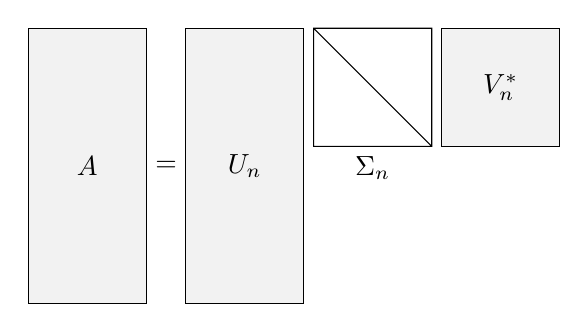
\begin{tikzpicture}[scale=0.5] 
  \draw[fill=black!5] (0,0) rectangle node {$A$} +(3,7);
  \node at (3.5,3.5) {=};
  \draw[fill=black!5] (4,0) rectangle node {$U_n$} +(3,7);
  \draw (7.25,4) rectangle +(3,3) (7.25,7) -- +(3,-3);
  \node[below] at (8.75,4) {$\Sigma_n$};
  \draw[fill=black!5] (10.5,4) rectangle node {$V_n^*$} +(3,3);
\end{tikzpicture}
\caption{\label{fig:svd}Scheme of the thin SVD of a rectangular matrix $A$.}
\end{figure}

In the following, we will assume that $m\geq n$. If $m<n$ then $A$ should be replaced by $A^*$ (note that in \slepc this is done transparently as described later in this chapter and the user need not worry about this). In the case that $m\geq n$, the top $n$ rows of $\Sigma$ contain $\mathrm{diag}(\sigma_1,\ldots,\sigma_n)$ and its bottom $m-n$ rows are zero. The relation \ref{eq:svd} may also be written as $AV=U\Sigma$, or
\begin{equation}
\label{eq:svdleft}
Av_i=u_i\sigma_i\;,\quad i=1,\ldots,n,
\end{equation}
and also as $A^*U=V\Sigma^*$, or
\begin{align}
\label{eq:svdright}
A^*u_i&=v_i\sigma_i\;,\quad i=1,\ldots,n,\\
\label{eq:svdright2}
A^*u_i&=0\;,\quad i=n+1,\ldots,m.
\end{align}
The last left singular vectors corresponding to Eq.\ \ref{eq:svdright2} are often not computed, especially if $m\gg n$. In that case, the resulting factorization is sometimes called the \emph{thin} SVD, $A=U_n\Sigma_n V_n^*$, and is depicted in Figure \ref{fig:svd}. This factorization can also be written as
\begin{equation}
\label{eq:svdouter}
A=\sum_{i=1}^{n}\sigma_iu_iv_i^*.
\end{equation}
Each $(\sigma_i,u_i,v_i)$ is called a singular triplet.

The singular values are real and nonnegative, $\sigma_1\geq\sigma_2\geq\ldots\geq\sigma_r>\sigma_{r+1}=\ldots=\sigma_n=0$, where $r=\mathrm{rank}(A)$. It can be shown that $\{u_1,\ldots,u_r\}$ span the range of $A$, $\mathcal{R}(A)$, whereas $\{v_{r+1},\ldots,v_n\}$ span the null space of $A$, $\mathcal{N}(A)$.

If the zero singular values are dropped from the sum in Eq.\ \ref{eq:svdouter}, the resulting factorization, $A=\sum_{i=1}^{r}\sigma_iu_iv_i^*$, is called the \emph{compact} SVD, $A=U_r\Sigma_r V_r^*$.

In the case of a very large and sparse $A$, it is usual to compute only a subset of $k\leq r$ singular triplets. We will refer to this decomposition as the \emph{truncated} SVD of $A$. It can be shown that the matrix $A_k=U_k\Sigma_k V_k^*$ is the best rank-$k$ approximation to matrix $A$, in the least squares sense. 

In general, one can take an arbitrary subset of the summands in Eq.\ \ref{eq:svdouter}, and the resulting factorization is called the \emph{partial} SVD of $A$. As described later in this chapter, \slepc allows the computation of a partial SVD corresponding to either the $k$ largest or smallest singular triplets.

\paragraph{Equivalent Eigenvalue Problems.}

It is possible to formulate the problem of computing the singular triplets of a matrix $A$ as an eigenvalue problem involving a Hermitian matrix related to $A$. There are two possible ways of achieving this:
\begin{enumerate}
\item With the \emph{cross product} matrix, either $A^*A$ or $AA^*$.
\item With the \emph{cyclic} matrix, $H(A)=\left[\begin{smallmatrix}0&A\\A^*&0\end{smallmatrix}\right]$.
\end{enumerate}
In \slepc, the computation of the SVD is always based on one of these two alternatives, either by passing one of these matrices to an \ident{EPS} object or by performing the computation implicitly.

By pre-multiplying Eq.\ \ref{eq:svdleft} by $A^*$ and then using Eq.\ \ref{eq:svdright}, the following relation results
\begin{equation}
\label{eq:eigleft}
A^*Av_i=\sigma_i^2v_i,
\end{equation}
that is, the $v_i$ are the eigenvectors of matrix $A^*A$ with corresponding eigenvalues equal to $\sigma_i^2$. Note that after computing $v_i$ the corresponding left singular vector, $u_i$, is readily available through Eq.\ \ref{eq:svdleft} with just a matrix-vector product, $u_i=\frac{1}{\sigma_i}Av_i$.

Alternatively, one could compute first the left vectors and then the right ones. For this, pre-multiply Eq.\ \ref{eq:svdright} by $A$ and then use Eq.\ \ref{eq:svdleft} to get
\begin{equation}
\label{eq:eigright}
AA^*u_i=\sigma_i^2u_i.
\end{equation}
In this case, the right singular vectors are obtained as $v_i=\frac{1}{\sigma_i}A^*u_i$.

The two approaches represented in Eqs.\ \ref{eq:eigleft} and \ref{eq:eigright} are very similar. Note however that $A^*A$ is a square matrix of order $n$ whereas $AA^*$ is of order $m$. In cases where $m\gg n$, the computational effort will favor the $A^*A$ approach. On the other hand, the eigenproblem \ref{eq:eigleft} has $n-r$ zero eigenvalues and the eigenproblem \ref{eq:eigright} has $m-r$ zero eigenvalues. Therefore, continuing with the assumption that $m\geq n$, even in the full rank case the $AA^*$ approach may have a large null space resulting in difficulties if the smallest singular values are sought. In \slepc, this will be referred to as the cross product approach and will use whichever matrix is smaller, either $A^*A$ or $AA^*$.

Computing the SVD via the cross product approach may be adequate for determining the largest singular triplets of $A$, but the loss of accuracy can be severe for the smallest singular triplets. The cyclic matrix approach is an alternative that avoids this problem, but at the expense of significantly increasing the cost of the computation. Consider the eigendecomposition of
\begin{equation}
\label{eq:cyclic}
H(A)=\left[\begin{matrix}0&A\\A^*&0\end{matrix}\right],
\end{equation}
which is a Hermitian matrix of order $(m+n)$. It can be shown that $\pm\sigma_i$ is a pair of eigenvalues of $H(A)$ for $i=1,\ldots,r$ and the other $m+n-2r$ eigenvalues are zero. The unit eigenvectors associated with $\pm\sigma_i$ are $\frac{1}{\sqrt{2}}\left[\begin{smallmatrix}\pm u_i\\v_i\end{smallmatrix}\right]$. Thus it is possible to extract the singular values and the left and right singular vectors of $A$ directly from the eigenvalues and eigenvectors of $H(A)$. Note that in this case singular values are not squared, and therefore the computed values will be more accurate. The drawback in this case is that small eigenvalues are located in the interior of the spectrum.

%---------------------------------------------------
\section{Basic Usage}

From the perspective of the user interface, the \ident{SVD} package is very similar to \ident{EPS}, with some differences that will be highlighted shortly.

\begin{figure}
\begin{Verbatim}[fontsize=\small,numbers=left,numbersep=6pt,xleftmargin=15mm]
SVD       svd;       /*  SVD solver context  */
Mat       A;         /*  problem matrix      */
Vec       u, v;      /*  singular vectors    */
PetscReal sigma;     /*  singular value      */
PetscInt  j, nconv;
PetscReal error;

SVDCreate( PETSC_COMM_WORLD, &svd );
SVDSetOperator( svd, A );
SVDSetFromOptions( svd );
SVDSolve( svd );
SVDGetConverged( svd, &nconv );
for (j=0; j<nconv; j++) {
  SVDGetSingularTriplet( svd, j, &sigma, u, v );
  SVDComputeError( svd, j, SVD_ERROR_RELATIVE, &error );
}
SVDDestroy( &svd );
\end{Verbatim}
\caption{\label{fig:ex-svd}Example code for basic solution with \ident{SVD}.}
\end{figure}

The basic steps for computing a partial SVD with \slepc are illustrated in Figure \ref{fig:ex-svd}. The steps are more or less the same as those described in chapter \ref{cap:eps} for the eigenvalue problem. First, the solver context is created with \ident{SVDCreate}. Then the problem matrix has to be specified with \ident{SVDSetOperator}. Then, a call to \ident{SVDSolve} invokes the actual solver. After that, \ident{SVDGetConverged} is used to determine how many solutions have been computed, which are retrieved with \ident{SVDGetSingularTriplet}. Finally, \ident{SVDDestroy} cleans up everything.

If one compares this example code with the \ident{EPS} example in Figure \ref{fig:ex-eps}, the most outstanding differences are the following:
\begin{itemize}
\item The singular value is a \texttt{PetscReal}, not a \texttt{PetscScalar}.
\item Each singular vector is defined with a single \texttt{Vec} object, not two as was the case for eigenvectors.
\item Function \ident{SVDSetOperator} only admits one \texttt{Mat} argument.
\item There is no equivalent to \ident{EPSSetProblemType}.
\end{itemize}
The reason for the last two differences is that \slepc does not currently support different kinds of SVD problems. This may change in future versions if some generalization of the SVD such as the GSVD is added.

%---------------------------------------------------
\section{Defining the Problem}

Defining the problem consists in specifying the problem matrix, $A$, and the portion of the spectrum to be computed. In the case of the SVD, the number of possibilities will be much more limited than in the case of eigenproblems.

The problem matrix is provided with the following function
	\findex{SVDSetOperator}
	\begin{Verbatim}[fontsize=\small]
	SVDSetOperator(SVD svd,Mat A);
	\end{Verbatim}
where \texttt{A} can be any matrix, not necessarily square, stored in any allowed \petsc format including the matrix-free mechanism (see \S\ref{sec:supported} for a detailed discussion).

It is important to note that all SVD solvers in \slepc make use of both $A$ and $A^*$, as suggested by the description in \S\ref{sec:svd}. $A^*$ is not explicitly passed as an argument to \ident{SVDSetOperator}, therefore it will have to stem from $A$. There are two possibilities for this: either $A$ is transposed explicitly and $A^*$ is created as a distinct matrix, or $A^*$ is handled implicitly via \ident{MatMultTranspose} (or \ident{MatMultHermitianTranspose} in the complex case) operations whenever a matrix-vector product is required in the algorithm. The default is to build $A^*$ explicitly, but this behavior can be changed with 
	\findex{SVDSetImplicitTranspose}
	\begin{Verbatim}[fontsize=\small]
	SVDSetImplicitTranspose(SVD svd,PetscBool impl);
	\end{Verbatim}

In \S\ref{sec:svd}, it was mentioned that in \slepc the cross product approach chooses the smallest of the two possible cases $A^*A$ or $AA^*$, that is, $A^*A$ is used if $A$ is a tall, thin matrix ($m\geq n$), and $AA^*$ is used if $A$ is a fat, short matrix ($m<n$). In fact, what \slepc does internally is that if $m<n$ the roles of $A$ and $A^*$ are reversed. This is equivalent to transposing all the SVD factorization, so left singular vectors become right singular vectors and vice versa. This is actually done in all singular value solvers, not only the cross product approach. The objective is to simplify the number of cases to be treated internally by \slepc, as well as to reduce the computational cost in some situations. Note that this is done transparently and the user need not worry about transposing the matrix, only to indicate how the transpose has to be handled, as explained above.

The user can specify how many singular values and vectors to compute. The default is to compute only one singular triplet. The function
	\findex{SVDSetDimensions}
	\begin{Verbatim}[fontsize=\small]
	SVDSetDimensions(EPS eps,PetscInt nsv,PetscInt ncv,PetscInt mpd);
	\end{Verbatim}
allows the specification of the number of singular values to compute, \texttt{nsv}. The second argument can be set to prescribe the number of column vectors to be used by the solution algorithm, \texttt{ncv}, that is, the largest dimension of the working subspace. These two parameters can also be set at run time with the options \Verb!-svd_nsv! and \Verb!-svd_ncv!. For example, the command line
\begin{Verbatim}[fontsize=\small]
	$ ./program -svd_nsv 10 -svd_ncv 24
\end{Verbatim}
requests 10 singular values and instructs to use 24 column vectors. Note that \texttt{ncv} must be at least equal to \texttt{nsv}, although in general it is recommended (depending on the method) to work with a larger subspace, for instance $\mathtt{ncv}\geq2\cdot\mathtt{nsv}$ or even more.
As in the case of the \ident{EPS} object, the last argument, \texttt{mpd}, can be used to limit the maximum dimension of the projected problem, as discussed in \S\ref{sec:large-nev}. Using this parameter is especially important in the case that a large number of singular values are requested.

\begin{table}
\centering
{\small \begin{tabular}{lll}
\texttt{SVDWhich}                  & Command line key                   & Sorting criterion \\\hline
\texttt{SVD\_LARGEST}   & \texttt{-svd\_largest}  & Largest $\sigma$ \\
\texttt{SVD\_SMALLEST}  & \texttt{-svd\_smallest} & Smallest $\sigma$ \\\hline
\end{tabular} }
\caption{\label{tab:whichsvd}Available possibilities for selection of the singular values of interest.}
\end{table}

	For the selection of the portion of the spectrum of interest, there are only two possibilities in the case of SVD: largest and smallest singular values, see Table \ref{tab:whichsvd}. The default is to compute the largest ones, but this can be changed with
	\findex{EPSSetWhichEigenpairs}
	\begin{Verbatim}[fontsize=\small]
	SVDSetWhichSingularTriplets(SVD svd,SVDWhich which);
	\end{Verbatim}
which can also be specified at the command line. This criterion is used both for configuring how the algorithm seeks singular values and also for sorting the computed values. In contrast to the case of \ident{EPS}, computing singular values located in the interior part of the spectrum is difficult, the only possibility is to use an \ident{EPS} object combined with a spectral transformation (this possibility is explained in detail in the next section). Note that in this case, the value of \Verb!which! applies to the transformed spectrum.

%---------------------------------------------------
\section{Selecting the SVD Solver}

The available methods for computing the partial SVD are shown in Table \ref{tab:svdsolvers}. These methods can be classified in the following three groups:
\begin{itemize}
\item Solvers based on \ident{EPS}. These solvers set up an \ident{EPS} object internally, thus using the available eigensolvers for solving the SVD problem. The two possible approaches in this case are the cross product matrix and the cyclic matrix, as described in \S\ref{sec:svd}.
\item Specific SVD solvers. These are typically eigensolvers that have been adapted algorithmically to exploit the structure of the SVD problem. There are currently two solvers in this category: Lanczos and thick-restart Lanczos. A detailed description of these methods can be found in the \hyperlink{str}{\slepc Technical Reports}.
\item The \lapack solver. This is an interface to some LAPACK routines, analog of those in the case of eigenproblems. These routines operate in dense mode with only one processor and therefore are suitable only for moderate size problems. This solver should be used only for debugging purposes.
\end{itemize}
The default solver is the one that uses the cross product matrix (\texttt{cross}), usually the fastest and most memory-efficient approach. See a more detailed explanation below.

\begin{table}
\centering
{\small \begin{tabular}{lll}
                           &                      & {\footnotesize Options} \\
Method                     & \ident{SVDType}      & {\footnotesize Database Name}\\\hline
Cross Product              & \texttt{SVDCROSS}    & \texttt{cross} \\
Cyclic Matrix              & \texttt{SVDCYCLIC}   & \texttt{cyclic} \\\hline
Lanczos                    & \texttt{SVDLANCZOS}  & \texttt{lanczos} \\
Thick-restart Lanczos      & \texttt{SVDTRLANCZOS}& \texttt{trlanczos} \\\hline
\lapack solver             & \texttt{SVDLAPACK}   & \texttt{lapack} \\\hline
\end{tabular} }
\caption{\label{tab:svdsolvers}List of solvers available in the \ident{SVD} module.}
\end{table}

The solution method can be specified procedurally or via the command line. The application programmer can set it by means of the command
	\findex{SVDSetType}
	\begin{Verbatim}[fontsize=\small]
	SVDSetType(SVD svd,SVDType method);
	\end{Verbatim}
while the user writes the options database command \Verb!-svd_type! followed by the name of the method (see Table \ref{tab:svdsolvers}).

The \ident{EPS}-based solvers deserve some additional comments. These SVD solvers work by creating an \ident{EPS} object internally and setting up an eigenproblem of type \ident{EPS\_HEP}. These solvers implement the cross product matrix approach, Eq.\ \ref{eq:eigleft}, and the cyclic matrix approach, Eq.\ \ref{eq:cyclic}. Therefore, the operator matrix associated with the \ident{EPS} object will be $A^*A$ in the case of the \texttt{cross} solver and $H(A)$ in the case of the \texttt{cyclic} solver.

In the case of the \texttt{cross} solver, the matrix $A^*A$ is not built explicitly, since sparsity would be lost. Instead, a shell matrix is created internally in the \ident{SVD} object and passed to the \ident{EPS} object. In the case of the \texttt{cyclic} solver, the situation is different since $H(A)$ is still a sparse matrix. \slepc gives the possibility to handle it implicitly as a shell matrix (the default), or to create $H(A)$ explicitly, that is, storing its elements in a distinct matrix. The function for setting this option is
	\findex{SVDCyclicSetExplicitMatrix}
	\begin{Verbatim}[fontsize=\small]
	SVDCyclicSetExplicitMatrix(SVD svd,PetscBool explicit);
	\end{Verbatim}

The \ident{EPS} object associated with the \texttt{cross} and \texttt{cyclic} SVD solvers is created with a set of reasonable default parameters. However, it may sometimes be necessary to change some of the \ident{EPS} options such as the eigensolver. To allow application programmers to set any of the \ident{EPS} options directly within the code, the following routines are provided to extract the \ident{EPS} context from the \ident{SVD} object,
	\findex{SVDCrossGetEPS}
	\findex{SVDCyclicGetEPS}
	\begin{Verbatim}[fontsize=\small]
	SVDCrossGetEPS(SVD svd,EPS *eps);
	SVDCyclicGetEPS(SVD svd,EPS *eps);
	\end{Verbatim}
A more convenient way of changing \ident{EPS} options is through the command-line. This is achieved simply by prefixing the \ident{EPS} options with \texttt{-svd\_} as in the following example:
\begin{Verbatim}[fontsize=\small]
	$ ./program -svd_type cross -svd_eps_type gd
\end{Verbatim}

At this point, one may consider changing also the options of the \ident{ST} object associated with the \ident{EPS} object in \texttt{cross} and \texttt{cyclic} SVD solvers, for example to compute singular values located at the interior of the spectrum via a shift-and-invert transformation. This is indeed possible, but some considerations have to be taken into account. When $A^*A$ or $H(A)$ are managed as shell matrices, then the potential of the spectral transformation is limited seriously, because some of the required operations will not be defined (this is discussed briefly in \S\ref{sec:supported} and \S\ref{sec:explicit}). Therefore, computing interior singular values is more likely to be successful if using the \texttt{cyclic} solver with explicit $H(A)$ matrix. To illustrate this, here is a complicated command-line example for computing singular values close to 12.0:
\begin{Verbatim}[fontsize=\small]
	$ ./program -svd_type cyclic -svd_cyclic_explicitmatrix -svd_st_type sinvert
                    -svd_eps_target 12.0 -svd_st_ksp_type preonly -svd_st_pc_type lu
\end{Verbatim}

%---------------------------------------------------
\section{Retrieving the Solution}

Once the call to \ident{SVDSolve} is complete, all the data associated with the computed partial SVD is kept internally in the \ident{SVD} object. This information can be obtained by the calling program by means of a set of functions described below.

As in the case of eigenproblems, the number of computed singular triplets depends on the convergence and, therefore, it may be different from the number of solutions requested by the user. So the first task is to find out how many solutions are available, with
	\findex{SVDGetConverged}
	\begin{Verbatim}[fontsize=\small]
	SVDGetConverged(SVD svd,PetscInt *nconv);
	\end{Verbatim}
Usually, the number of converged solutions, \texttt{nconv}, will be equal to \texttt{nsv}, but in general it will be a number ranging from 0 to \texttt{ncv} (here, \texttt{nsv} and \texttt{ncv} are the arguments of function \ident{SVDSetDimensions}).

Normally, the user is interested in the singular values only, or the complete singular triplets. The function
	\findex{SVDGetSingularTriplet}
	\begin{Verbatim}[fontsize=\small]
	SVDGetSingularTriplet(SVD svd,PetscInt j,PetscReal *sigma,Vec u,Vec v);
	\end{Verbatim}
returns the $j$-th computed singular triplet, $(\sigma_j,u_j,v_j)$, where both $u_j$ and $v_j$ are normalized to have unit norm. Typically, this function is called inside a loop for each value of \texttt{j} from 0 to \texttt{nconv}--1. Note that singular values are ordered according to the same criterion specified with function \ident{SVDSetWhichSingularTriplets} for selecting the portion of the spectrum of interest.

In some applications, it may be enough to compute only the right singular vectors. This is especially important in cases in which memory requirements are critical (remember that both $U_k$ and $V_k$ are dense matrices, and $U_k$ may require much more storage than $V_k$, see Figure \ref{fig:svd}). In \slepc, there is no general option for specifying this, but the default behavior of some solvers is to compute only right vectors and allocate/compute left vectors only in the case that the user requests them. This is done in the \texttt{cross} solver and in some special variants of other solvers such as one-sided Lanczos (consult the \slepc \hyperlink{str}{technical reports} for specific solver options).

\paragraph{Reliability of the Computed Solution.}

In SVD computations, a-posteriori error bounds are much the same as in the case of Hermitian eigenproblems, due to the equivalence discussed in \S\ref{sec:svd}. The residual vector is defined in terms of the cyclic matrix, $H(A)$, so its norm is
\begin{equation}
\|r\|_2=\left(\|A\tilde{v}-\tilde{\sigma}\tilde{u}\|_2^2+\|A^*\tilde{u}-\tilde{\sigma}\tilde{v}\|_2^2\right)^{\frac{1}{2}},
\end{equation}
where $\tilde{\sigma}$, $\tilde{u}$ and $\tilde{v}$ represent any of the \texttt{nconv} computed singular triplets delivered by \texttt{SVDGetSingularTriplet}.

Given the above definition, the following relation holds
\begin{equation}
|\sigma-\tilde{\sigma}|\leq \|r\|_2,
\end{equation}
where $\sigma$ is an exact singular value. The associated error can be obtained in terms of $\|r\|_2$ with the following function:
	\findex{SVDComputeError}
	\begin{Verbatim}[fontsize=\small]
	SVDComputeError(SVD svd,PetscInt j,SVDErrorType type,PetscReal *error);
	\end{Verbatim}

\paragraph{Controlling and Monitoring Convergence.}

Similarly to the case of eigensolvers, in \ident{SVD} the number of iterations carried out by the solver can be determined with \ident{SVDGetIterationNumber}, and the tolerance and maximum number of iterations can be set with \ident{SVDSetTolerances}. Also, convergence can be monitored with command-line keys \Verb!-svd_monitor!, \Verb!-svd_monitor_all!, \Verb!-svd_monitor_conv!, \Verb!-svd_monitor_lg!, or \Verb!-svd_monitor_lg_all!. See \S\ref{sec:monitor} for additional details.

\paragraph{Viewing the Solution.}

There is support for different kinds of viewers for the solution, as in the case of eigensolvers. One can for instance use \Verb!-svd_view_values!, \Verb!-svd_view_vectors!, \Verb!-svd_error_relative!, or \Verb!-svd_converged_reason!. See description in \S\ref{sec:epsviewers}.

